\documentclass{standalone}
\usepackage{pgfplots}
\pgfplotsset{compat=newest}

\begin{document}
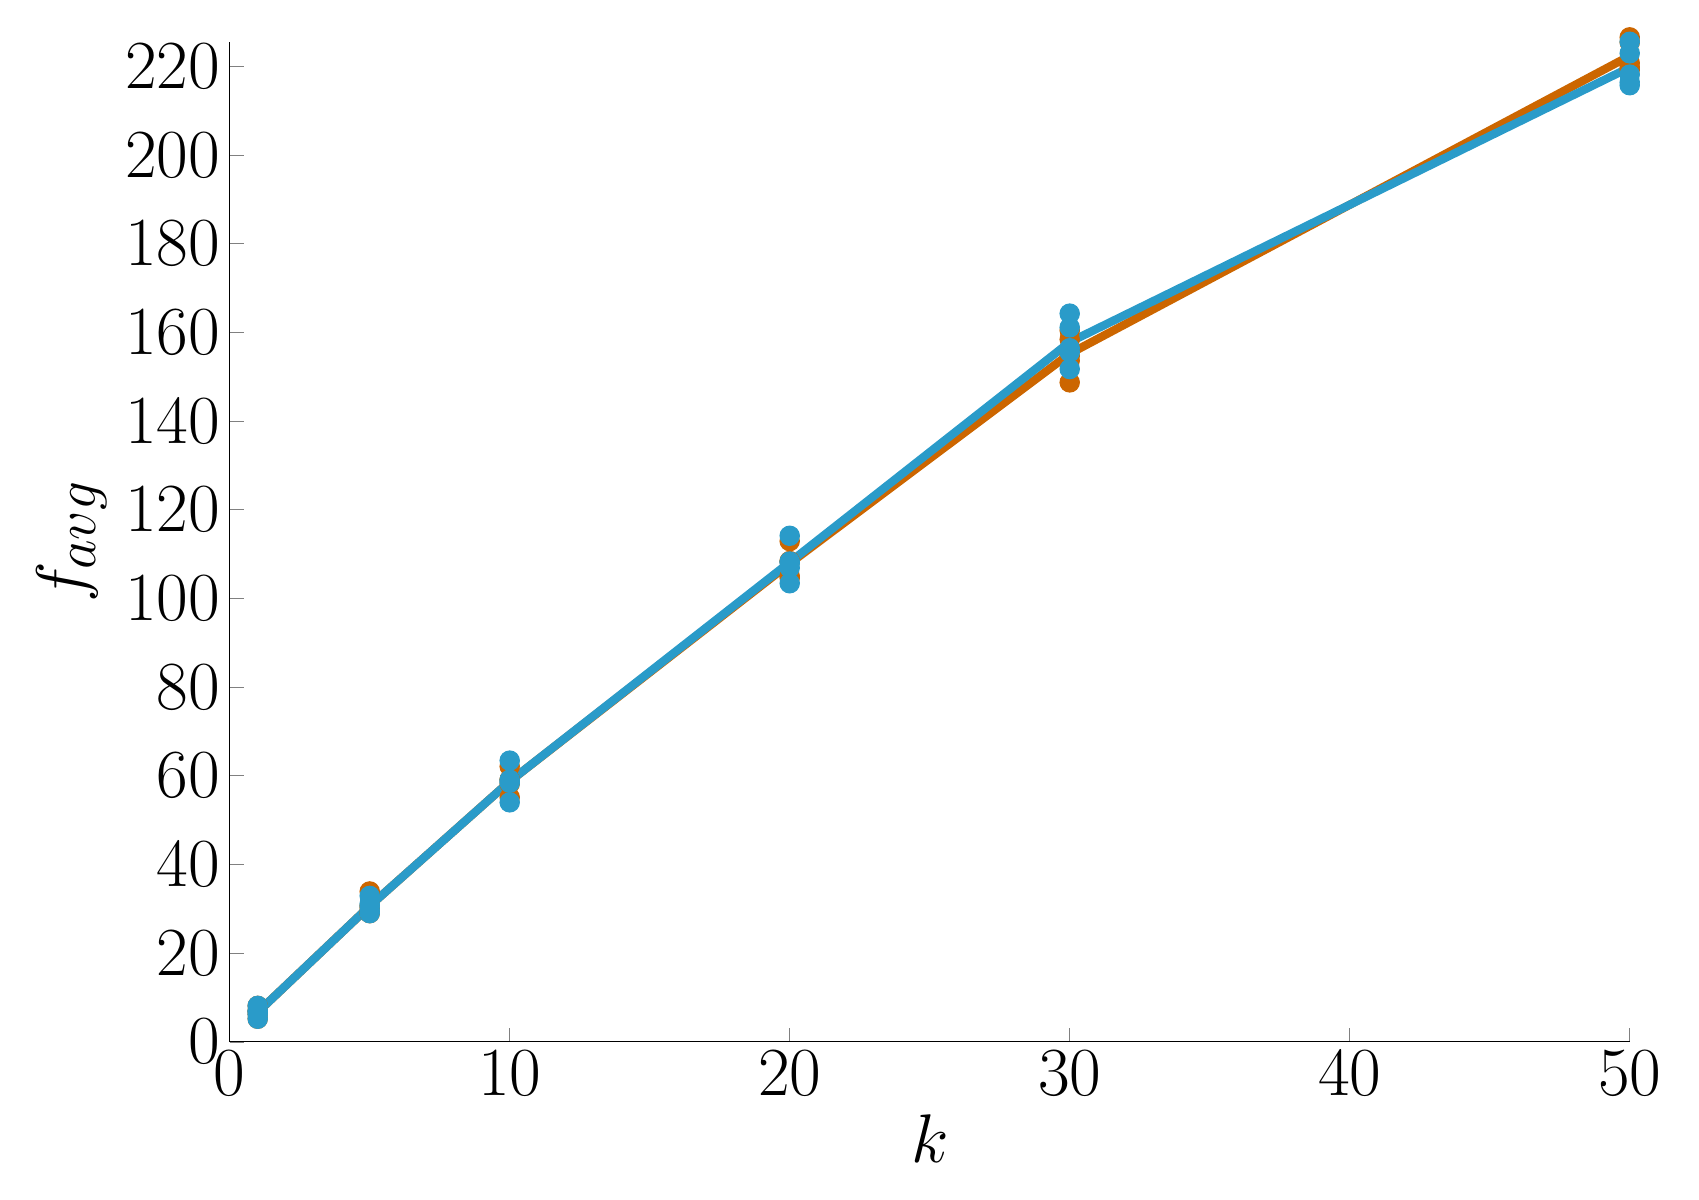
\begin{tikzpicture}

\begin{axis}[%
tick label style={font=\Huge},
label style={font=\Huge},
legend style={font=\Huge},
view={0}{90},
max space between ticks=50pt,
width=7in,
height=5in,
scale only axis,
xmin=0, xmax=50,
xtick={0, 10, 20, 30, 40, 50},
xlabel={$k$},
ymin=0, ymax=225.5,
%ytick={0, 200, 400, 600, 800, 1000},
ylabel={$f_{avg}$},
major tick length=5pt,
axis lines*=left,
legend cell align=left,
clip=false]

\addplot [
only marks,
mark=*,
mark size=3.5pt,
color=orange!80!black,
%solid,
%line width=2pt,
]
coordinates{
(1,5.2)(1,6.2)(1,6.8)(1,7.0)(1,8.1)(5,29.0)(5,29.3)(5,30.2)(5,30.7)(5,33.9)(10,55.1)(10,58.2)(10,59.1)(10,59.1)(10,62.1)(20,104.6)(20,105.0)(20,108.3)(20,108.4)(20,112.9)(30,148.7)(30,153.6)(30,154.7)(30,158.4)(30,160.4)(50,219.2)(50,219.8)(50,220.7)(50,225.4)(50,226.5)
};

\addplot [
only marks,
mark=*,
mark size=3.5pt,
color=cyan!80!black,
%solid,
%line width=2pt,
]
coordinates{
(1,5.2)(1,6.2)(1,6.8)(1,7.0)(1,8.1)(5,29.0)(5,29.6)(5,30.5)(5,31.1)(5,32.9)(10,54.0)(10,58.4)(10,58.7)(10,59.1)(10,63.4)(20,103.4)(20,106.9)(20,108.0)(20,108.3)(20,114.1)(30,151.7)(30,155.5)(30,156.4)(30,161.1)(30,164.2)(50,215.7)(50,216.4)(50,218.1)(50,222.9)(50,225.5)
};

\addplot [
color=orange!80!black,
solid,
line width=3pt
]
coordinates{
(1,6.66)(5,30.62)(10,58.72)(20,107.84)(30,155.16)(50,222.32)
};

\addplot [
color=cyan!80!black,
solid,
line width=3pt
]
coordinates{
(1,6.66)(5,30.62)(10,58.72)(20,108.14)(30,157.78)(50,219.72)
};


\end{axis}
\end{tikzpicture}
\end{document}
